\documentclass[a4paper,11pt]{article}
\usepackage{graphicx}
\usepackage{wrapfig}
\usepackage[a4paper, inner=3cm, outer=3cm, top=3cm, bottom=3cm, offset=0cm]{geometry}
\author{Kenneth Cross}
\title{\textbf{Scheduling Algorithm}}
\date{\today}

\begin{document}
\pagenumbering{gobble}
\maketitle
\newpage
\tableofcontents
\newpage
\pagenumbering{arabic}
\setcounter{page}{1}

\newpage

\section{Methodology}

1) Staff Generation: Stored in a possibility matrix
2) Staff Optimization
3) Schedule Based on Staff Optimization Sum
4) Schedule Satisfaction Optimization

Maximization Factors
* Localization: establish potential rhythms and patterns for objects
* Position Preference: establish staff shift preferences
* Employee Preference: establish a hierarchy of skill based labor and give preference of desirable shifts to skilled employees. 

Multiple Shift Additions: Morning, Afternoon, Graveyard aka MAG

\begin{wrapfigure}{r}{4.5cm}
    \includegraphics[height=10cm]{graph.eps}
    \caption{\small Algorithm Digraph}
\end{wrapfigure}

\section{Modules and Functions}

The entire depth of the inner workings of the program/algorithm are outlined here. 
The subsections try to follow a logical working order of pragmatic flow.

\subsection{Roster Initializations}
\subsection{Workday Validation}
\subsection{Rostering Optimizations}
\subsection{Scheduler Optimizations}
\subsection{Multi-Shift Support}

This should be taken care of in the scheduler algorithm rather than the rostering algorithm.
This makes sense because rostering will calculate all possibilities of a person's availability rather than overlook other possibilities for other shifts.
The scheduler should have a section to combine and compare full shift schedules where logic should be performed for optimizations and shifting conflicts or other legal parameters.

\subsection{Multi-Shift Optimizations}

\section{Data Representations}

Incoming input is currently contained in two separate CSV files. 
One file contains employee availability where the position section is a preference as to how many times per week someone would like to perform that position. The other file contains what types of positions are required and how many of each for every day of the week.


\end{document}
